% vim: spell spl=hu
\section{A blAST architektúrája}

Ebben a fejezetben a blAST rendszer felépítését tárgyalom.
A tárgyalás a felhasználó számára látható nyelvi elemektől indul, és a tényleges kiértékelőig tart.

A blAST három lényegi rétegből áll: az első a \gls{eDSL} réteg, amelyik C4 kódban teszi lehetővé a keresések leírását; a második a C4--C--C++ konverziós réteg, aminek a feladata hogy a C4-ben létrehozott keresések a Clang \gls{API} megfelelő részeire eljussanak; végül a végrehajtó réteg.

\subsection{Az \glslink{eDSL}{eDSL} réteg}

Az \gls{eDSL} réteg meglepően egyszerű strukturálisan: lényegében csak a lustán kiértékelt függvények megfelelő módú kompozíciójából áll elő a kívánt szintaktika.
Minden konkrét szintaktikai elem, egy olyan függvény, amelyik maga is egy blokk (lambda) értékével tér vissza.
Ezek a blokkok azok, amelyek képesek lesznek arra, hogy előállítsanak egy olyan szöveges ASTMatcher leírást, amelyiket után lehetséges a végrehajtó réteg számára átadni.

Ez a logika valamelyes hasonlít olyan SQL generátor eszközökre, amelyek a gazdanyelv függvényein keresztül állítanak elő SQL lekérdezéseket.
Ilyen \pl a Ruby on Rails keretrendszer ActiveRecord objektum--relációs leképező könyvtára által használt ARel könyvtár \todo{Cite RoR's AR}.

Ehhez a belső függvények általában 5 paraméterrel dolgoznak, de kettő fontos: a jelenlegi ASTMatcher példányokat leíró függvények listája ({\tt ms}) és a találatokat kezelő kódrészletek listája ({\tt hs}).
A többi paramétert néha nem használják fel -- mint az alábbi példában sem az {\tt any} nevű paramétert.
Ebbe a két paraméterbe azonban, megfelelő módon átadva azokat vagy belső segédfüggvényeknek, vagy további hívott \gls{eDSL} elemeknek, fűzik a lépésenként létrehozott adatokat.
A folyamat végén egy olyan dinamikus hívás áll, amelyik az {\tt ms} listából sztringeket, az {\tt hs} listából pedig kezelő objektumokat kap.
Utóbbiakat a következő szakasz tárgyalja, mivel nagy részben a C++ kód konverzióját veszi igénybe a C4 futtatókörnyezetbe.

\Aref{lst:blast-call}.~listázás valósítja meg azt a \cfn call/1 függvényt, amelyik a függvényhívás kifejezéseket teszi lehetővé megkeresni \pl a {\tt any call expression} C4 kifejezésben.
Ezen a lényegi része az előbb bemutatott elemeknek látszik: a külső függvény átveszi a belső függvény \pl az \cfn expression/0 még ki nem értékelt értékét, és egy olyan blokk érték formájában adja vissza, amelyik meghívja azt.
Ennek továbbadja az alap 5 paramétert, amelyből a saját {\tt "callExpr"} értékkel felül ír egyet: ez fogja a tényleges \cfn expression/0 kódjában az alapértelmezett {\tt "expr"} részt lecserélni.
A {\tt body} a \cfn such/2 függvény szűrői lehetnek, míg a {\tt bondage} a \cfn bound/2 függvény (vagy az ekvivalens operátor) által hozzá kötött elnevezése az \gls{AST} elemnek.

\begin{lstlisting}[label={lst:blast-call},caption=Példa a blAST \gls{eDSL} megvalósításából]
let +call/1 { |m| { |ms hs any body bondage|
	&(m)/5 ms hs "callExpr" body bondage
}}
\end{lstlisting}

Ennek a felépítésnek köszönhető a könnyű komponálhatósága az egyes lekérdezéseknek, amit az előző szakasz végén be is mutattam.
Mivel egy adott szintaktikai elem egyedüli feladat, hogy egy olyan függvényt adjon vissza, amelyik megfelel hívó kód elvásárainak, így a publikus függvények szabad komponálásán keresztül ez teljesül.

A \cfn blast/2 függvény összesen csak ezt a hívási láncot kezdeményezi, majd a létrejött kereső és kezelő listákat átadja a natív kód számára, amelyik végrehajtja azt.
Ehhez nyilván az általa kapott AST definíciót is továbbadja.

\subsection{A konverziós réteg}

A konverziós réteg feladata, hogy a dinamikusan típusos C4 értékekből megfelelő formátumú Clang objektumokat hozzon létre.
Ehhez a C4 nyelv megvalósításának egy speciális tulajdonságát használja ki: az alaptípusok mellett van egy csak a C oldalról elérhető típus: ``C4\_External''.
Ennek a teljes létjogosultsága, hogy a C4 futtatókörnyezet számára átlátszatlan ({\tt opaque}) módon lehessen saját értékeket tárolni különböző \gls{DSL} megvalósítások számára.
Ezt a lehetőséget használja a blAST is.

Fontos említeni, hogy ennek a rétegnek a feladata bonyolultabb, mint elsőre tűnhet: ennek oka, hogy igazából $3$ irányban kell fordítani: a dinamikusan típusos, lusta C4 nyelv immutábilis értékei, a C procedurális struktúrákba rendezett adatai, és végül a Clang által használt, mélyen objektum-orientált C++ objektumok között.
Az élettartamokra kiemelkedően: a C4 értékek automata szemétgyűjtővel (\gls{GC}) kerülnek kezelésre, a C adatok manuálisan takarítandóak fel, míg a Clang C++ objektumok gyakran a \gls{RAII} elvet követő erőforrás kezelő típusokba van rendezve.
Utóbbinak extra nehézségeiről a következő paragrafusok még megemlékeznek.

A folyamat magában egyszerű: az első használatakor egy ilyen saját külső típusnak, el kell kérni egy adott futás során egyedi azonosítót az új típus számára.
Ez egy 32-bites előjel nélküli szám, így $2^{32}-2$ darab egyedi típus lehet (a $0$ a nem meghatározott azonosítót képviseli) egy lefutás során.
Ezeknek a neve altípus (subtype), mert az érték elsődleges típusa marad ``C4\_External''.
Az összes altípust azonosan kezeli az alap C4 rendszer: mintha egy blokk típusú érték lenne, bármilyen művelet számára csak a mutató értékeként kerül felhasználásra.
Ez biztosítja, hogy a külső érték mindig helyesen megmarad a egyéb C4 kód futása közben.

A konverziós réteg ezekből az altípusokból három fajtát regisztrál be: 1) a fordítási adatbázis, 2) az \gls{AST} egység ({\tt clang::\bf ASTUnit}) és 3) a találatokat lekezelő (handler) típus.
Ezek összességében alkotják a C++ elemeit a blAST rendszernek, amelyeket ez a réteg fordít C4\_External értékekből konkrét, helyesen típusos C++ objektumokká.

\paragraph{Az adatbázis}
Az előző fejezetben említett fordítási adatbázisokat a Clang libTooling alapú eszközökben a {\tt clang::tooling::{\bf CompilationDatabase}} osztály és leszármazottjai kezelik.
Ennek a hierarchiának kerül kiosztásra az egyik altípus.
Az alábbiakban tárgyalt \gls{GC} finalizer függvénye itt is releváns a destruktor meghívására, de itt konkrét értékként megkapható az objektum, úgyhogy az alábbi dupla indirekció elkerülhető.

\paragraph{Az ASTUnit}
A Clang könyvtárak egyik alapvető osztálya a {,,{\tt clang::\bf ASTUnit}''}.
Ez tárolja magában azokat a fordítási egységeket (\gls{TU}), amelyeket már a fordító elemzett és egy \gls{AST}-t készített belőle.
A blAST rendszerben van lehetőség pusztán fájlokat elemezni, nem csak teljes projekteket.
Ennek megvalósításra használja ezeket az objektumokat: a C4 kódban megadott forrásfájlból készült \gls{AST} egyég így jut el az elemzés fázisig.

Az előzőekben említett extra nehézség itt jelenik meg: az egységek okos mutatókban ({\it smart pointer}) kérhetőek csak le.
Ez normális esetben jó, mert megoldják a fejlesztő helyett az erőforrások kezelését.
Itt azonban problémás, mert a tényleges {\tt ASTUnit} objektumot a C4 \gls{GC} hatálya alá kell helyezni, mert addig életben kell tartani, amíg maga a C4 érték hivatkozik rá.

\begin{figure}[htb]
\centering
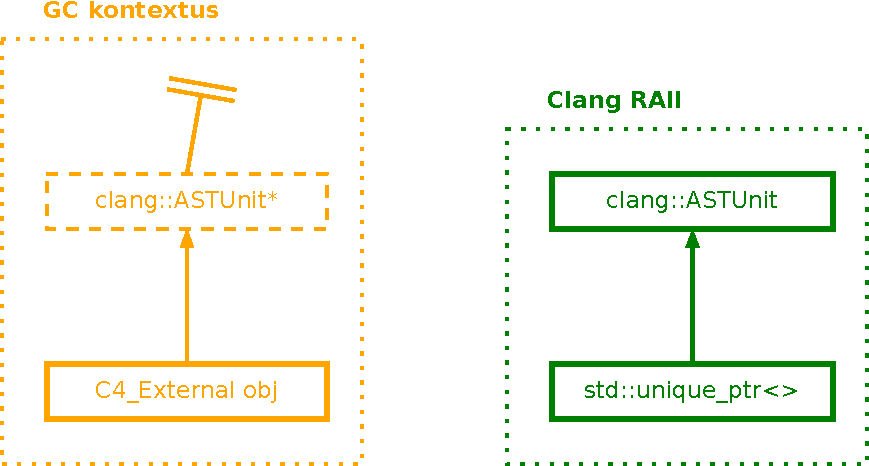
\includegraphics[width=.67\linewidth]{figures/smart.pdf}
\vskip1em
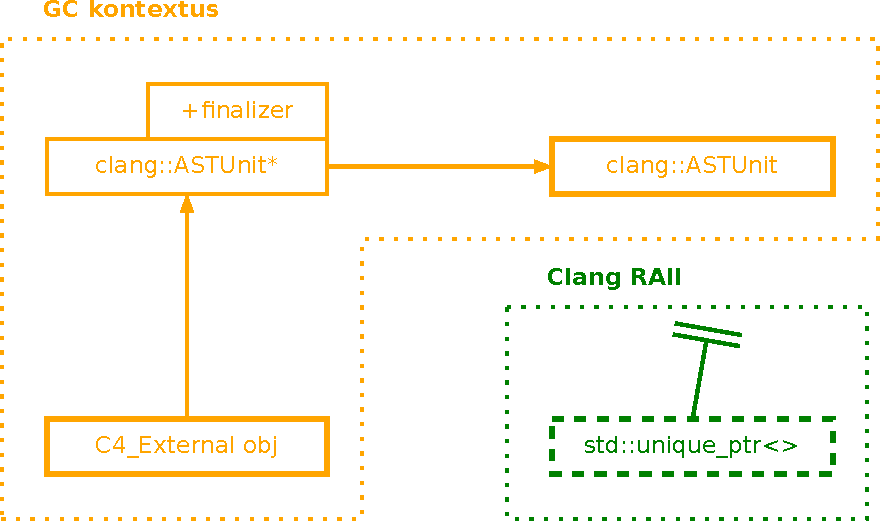
\includegraphics[width=.67\linewidth]{figures/gc.pdf}
\caption{A Clang \gls{RAII} értékek \gls{GC} alá helyezése}
\label{fig:raii2gc}
\end{figure}

Ennek a műveletnek a lefolyása látszik \aref{fig:raii2gc}.~ábrákon.
A visszakapott mutató számára egy külön mutató érték kerül lefoglalásra.
Erre azért van szükség, mert a C4 érték mutatójának helyére kellene a tényleges C++ objektumot mozgatni/másolni.
Az objektumnak azonban nincsenek megfelelő konstruktorai -- marad tehát a kétszeres indirekció.
Fontos kiemelni a destruktorok kezelését.
Az objektum determinisztikus C++ destruktorát át kell emelni a nem-determinisztikus \gls{GC} világba, amire a finalizer függvény nyújt lehetőséget.
Itt egy megfelelően \gls{GC} számára beregisztrált C++ lambdába csomagolt {\tt std::{\bf destruct\_at}()} függvény teszi lehetővé megbízhatóan destruktorok hívását egy-egy memóriacímen.

\paragraph{A handler osztályok}
A handler osztályok feladata, hogy a sikeresen megtalált \gls{AST} elemeket a megfelelő módon lekezeljék.
Ez egy egyszerű osztály-hierarchián keresztül kerül megvalósításra: a {\tt callback\_handler} leszármazott osztály feladata, a felhasználó által megadott C4 kódrészletek lefuttatása az egyes talált értékekre.
Bár igazából ez elég minden további megvalósításra, hatékonysági és keresés-fejlesztői kényelem szempontjából a {\tt diagnostic\_handler} osztály biztosít egy specifikusan egy diagnosztikai üzenet kiírását megvalósító kezelőt.
Az \cfn ignored/0 kezelőt az {\tt ignore\_handler} valósítja meg, semmilyen művelettel.

Egy összefoglaló, egyszerűsített mezőket tartalmazó osztálydiagram látható \aref{fig:handlers}.~ábrán.
Az egyes megjegyzések egy nagyon leegyszerűsített pszeudokódot mutatnak a fontosabb függvényekhez, amik segítenek a viselkedés értelmezésében.

Ezeket az elemeket használják az előzőekben már említett és bemutatott \cfn callback/1 és \cfn diagnostic/1 C4 függvények.
Meghívásukkor létrehozzák a megfelelő objektumot, majd a C4 \gls{GC} számára elérhetővé teszik a megfelelő címet.
Ezek az osztályok saját fejlesztésűek, így az előbbiekben említtet {\tt clang::\bf ASTUnit}-al ellentétben, itt direkt módon lehetséges egy placement new kifejezéssel a \gls{GC} memória címterébe létrehozni a objektumokat.
Ennek előnye, hogy kevesebb az indirekció miatti mutató kergetés (pointer chasing).

\begin{figure}[htb]
\centering
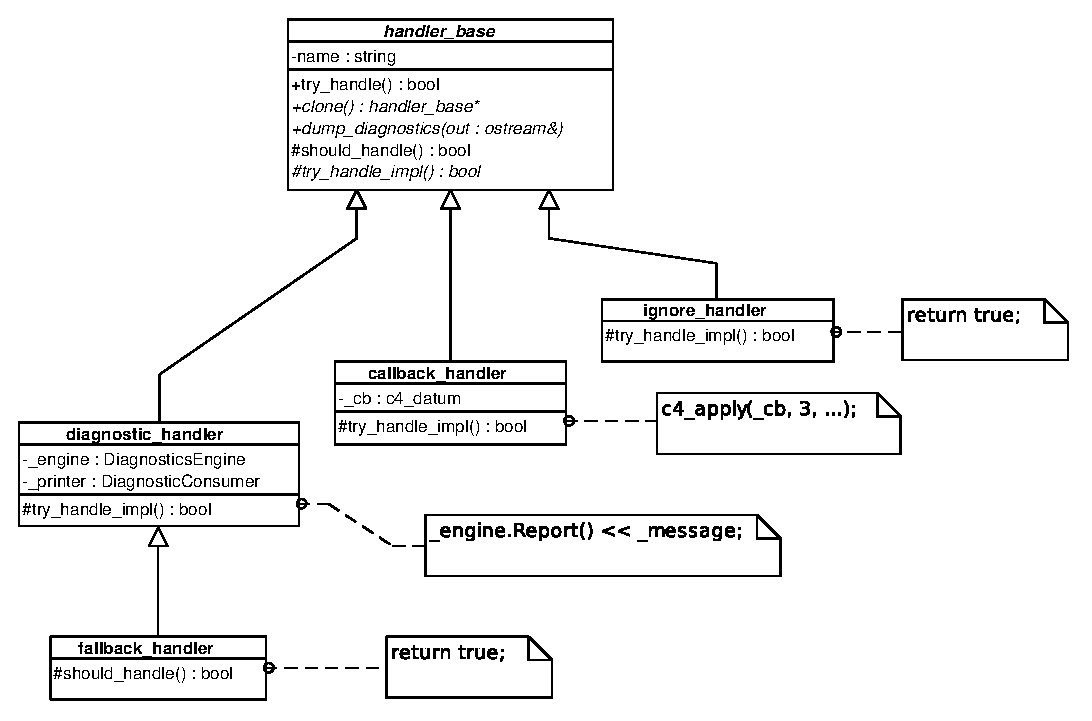
\includegraphics[width=.8\linewidth]{figures/handlers.eps}
\caption{A handler osztályok osztálydiagramja}
\label{fig:handlers}
\end{figure}

\subsection{A végrehajtó réteg}

Az első két réteg után, a végrehajtó réteg feladata már javarészt C++ kódként jelenik meg.
Miután a C4 interfészből beérkező adatok kicsomagolása megtörtént, teljesen normális C++ kódnak hat a tényleges megvalósítás is.

A tényleges futtatáshoz előre létrehozott szálakat használ a blAST.
Ezek darabszáma az elvégzendő feladatok (forrásfájlok, amelyeket ellenőrizni kell) és a futtató hardver kapacitásától függ.
A tényleges munkamegosztás kiemelkedően egyszerű, mert triviálisan párhuzamosítható: minden adott forrásfájl ellenőrzése független az összes többi forrásfájltól.
Ezt a jó tulajdonságát a C fordítási modelljének köszönheti, mert ugyanúgy, ahogy a fordító számára függetlenek az egyes forrásokból előállított objektumfájlok, az analízis eszköz számára is csak a konkrét forrás \gls{AST} leírására van szüksége.
A fejlécfájlokat itt most nem tekintjük külön forrásnak, hiszen a bennük található kódot amúgy is megtalálja az eszköz az {\tt\#include} direktívákon keresztül.

Minden munkavégző szál kap egy saját {\tt clang::ast\_matchers::\bf MatchFinder} példányt, és egy dinamikusan kezelt sztringet, amelyikbe gyűjtheti az általa talált eredményeket.
Fontos a párhuzamosítás miatt, hogy ne menet közben írjuk ki ezeket, mert különben összekavarodhatnak az adott szálakról szóló kimenetek.

Mivel maguk a matcher példányok nem változnak keresés közben, így ezeket meg tudják osztani egymás között a szálak.
Ezeket a objektumokat kapják meg a saját szál által kezelt {\tt MatchFinder} objektumok.

A konkrét forrásokat egy közös, zárolt, sorból veszik ki.
Egy egyszerűség, hogy ez előre ismert.
Emiatt ez egyszer feltöltődik a futás elején, majd több fogyasztó (itt a munkavégző szálak) egyesével veszik ki belőle a forrásokat, amit lefuttatják az ellenőrzéseket.
Ez látszik \aref{fig:threads}.~ábrán: minden szál a következő forrásfájlt kiveszi, majd a saját {\tt MatchFinder} felhasználásával a keresett mintákat megkeresi benne.

\begin{figure}
\centering
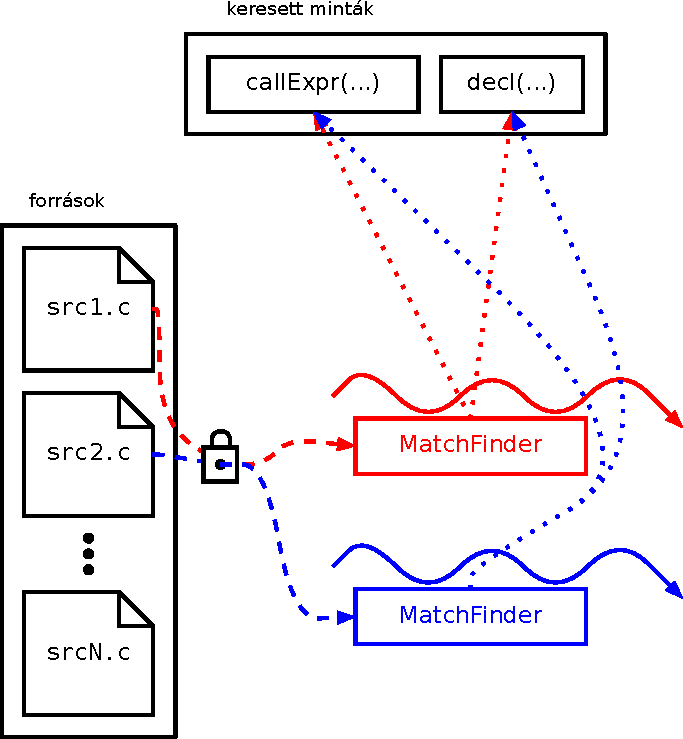
\includegraphics[width=.7\linewidth]{figures/threads.pdf}
\caption{A blAST szálak összedolgozása}
\label{fig:threads}
\end{figure}

